% Figura: Extended Pipeline Architecture
\begin{figure}[!htb]
\centering
\resizebox{0.85\columnwidth}{!}{%
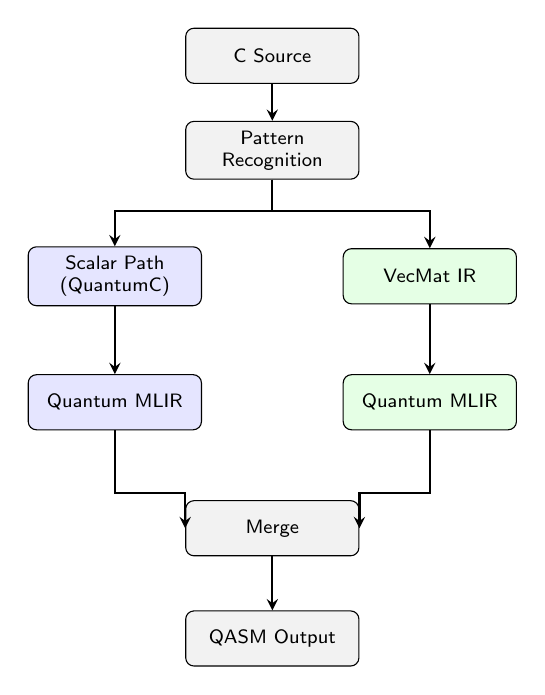
\begin{tikzpicture}[
    box/.style={
        draw,
        rounded corners=3pt,
        minimum width=2.2cm,
        minimum height=0.7cm,
        align=center,
        font=\sffamily\scriptsize
    },
    mainbox/.style={box, fill=gray!10},
    scalarbox/.style={box, fill=blue!10},
    vecbox/.style={box, fill=green!10},
    arrow/.style={->, >=stealth, thick}
]

% Riga 0: C Source
\node[mainbox] (source) at (0, 0) {C Source};

% Riga 1: Pattern Recognition
\node[mainbox] (pattern) at (0, -1.2) {Pattern\\Recognition};

% Riga 2: Branch - due path
\node[scalarbox] (scalar) at (-2, -2.8) {Scalar Path\\(QuantumC)};
\node[vecbox] (vecmat) at (2, -2.8) {VecMat IR};

% Riga 3: Entrambi producono Quantum MLIR
\node[scalarbox] (sqmlir) at (-2, -4.4) {Quantum MLIR};
\node[vecbox] (vqmlir) at (2, -4.4) {Quantum MLIR};

% Riga 4: Merge
\node[mainbox] (merge) at (0, -6.0) {Merge};

% Riga 5: QASM Output
\node[mainbox] (qasm) at (0, -7.4) {QASM Output};

% === FRECCE ===

% Top: source -> pattern
\draw[arrow] (source) -- (pattern);

% Branch: pattern -> scalar e pattern -> vecmat
\draw[arrow] (pattern.south) -- ++(0, -0.4) -| (scalar.north);
\draw[arrow] (pattern.south) -- ++(0, -0.4) -| (vecmat.north);

% Scalar path: scalar -> sqmlir
\draw[arrow] (scalar) -- (sqmlir);

% Vector path: vecmat -> vqmlir (lowering diretto)
\draw[arrow] (vecmat) -- (vqmlir);

% Convergenza verso Merge
\draw[arrow] (sqmlir.south) -- ++(0, -0.8) -| (merge.west);
\draw[arrow] (vqmlir.south) -- ++(0, -0.8) -| (merge.east);

% Bottom: merge -> qasm
\draw[arrow] (merge) -- (qasm);

\end{tikzpicture}%
}
\caption{Extended QuantumC compilation pipeline. The scalar path follows the original QuantumC stages, while the vector/matrix path processes recognized patterns through the VecMat IR with direct lowering to quantum operations.}
\label{fig:pipeline}
\end{figure}
